\section{Daten}
Dieses Kapitel geht darauf ein, woher wir die Daten für das Training des Netzes beschaffen und wie wir diese vor-bearbeiten.

\subsection{Quelle}
Die verwendeten Daten stammen vom Deutschen Wetterdienst (ab jetzt DWD) und sind Radardaten von deren Radarstationen. Die Daten der Messstationen bilden Kreise um die jeweiligen Stationen und bedecken noch einen kleinen Bereich um Deutschland; die Daten geben die Stärke des Niederschlags an. Die Radar-Messungen liegen in einer Auflösung von einer Stunde und 5 Minuten vor, wir verwenden letztere. Z.zt. liegen die Daten vom Januar 2001 bis Januar 2018 vor (jeweils inklusive). Für unsere Zwecke verwenden wir die 18 kompletten Jahre 2001 bis 2017.\footnote{\url{https://opendata.dwd.de/climate\_environment/CDC/grids\_germany/5\_minutes/radolan/reproc/2017\_002/bin/}}

\subsubsection{Crawler}
Da die Daten in monatsweise in geschachtelten Archiven gepackt sind, haben wir einen Crawler geschrieben, der die Daten zuerst herunterlädt und auspackt. Mit den Kommandozeilenoptionen\footnote{\url{https://github.com/thgnaedi/DeepRain/tree/master/DWD_Crawler}} kann gesteuert werden, ob die stündlichen oder minütlichen Daten heruntergeladen werden und wohin die Binärdateien entpackt werden sollen. Wir empfehlen, die Binärdaten auf eine Btrfs\footnote{\url{https://en.wikipedia.org/wiki/Btrfs}}-formatierte Partition zu entpacken, da die Daten (wegen häufig auftretender Nullen bzw. kein Regen) leicht komprimierbar sind und die minütlichen Daten sonst mehr als ein Terabyte belegen würden.

\subsection{Preprocessing}
Um das Binärformat des DWD einzulesen, benötigt man die Python-Bibliothek \gqq{Wradlib}, die man über den Package-Manager von Anaconda installieren kann. Dann kann man die Datensätze als Deutschlandkarte mit einer Auflösung von 1100x900 Pixeln rastern.

Das Preprocessing geschieht in zwei Durchläufen: Zuerst wird das Maximum des Niederschlags bestimmt, das Minimum wird als 0 (kein Regen) angenommen. Danach werden die Werte auf einen Bereich gespreizt.

Beim zweiten Durchgang werden die Daten mithilfe des globalen Maximalwertes auf einen Wertebereich zwischen 0 und 255 umgerechnet, damit die Datensätze in einem Bildformat mit einer Bittiefe von 8 Bit gespeichert zur weiteren Verarbeitung werden können. Wir haben uns für das PNG-Format entschieden, weil es verlustfrei komprimiert und von platt­form­über­grei­fenden Bibliotheken gelesen und geschrieben werden kann.
Vor dem Speichern werden die Werte mit dem Faktor 4 multipliziert um Werte über 255 auf den Maximalwert abzuschneiden. Dadurch verwerfen wir Ausreißer und das Training funktioniert besser. Der Faktor 4 wurde empirisch bestimmt, weil das Berechnen eines Histogramms über alle 18 Jahre zu aufwendig gewesen wäre.

\subsubsection{Trainingsdaten}
\label{Samples}
Da sich unsere Aufgabenstellung mit einer Regenvorhersage für Konstanz befasst, sind die aktuell gespeicherten Bilder noch deutlich zu groß. Daher wird aus dem gespeicherten Bild nur ein kleiner Bereich um Konstanz herum ausgeschnitten. die Position von Konstanz wurde bereits zuvor in Kapitel \ref{locKN} bestimmt. Um diese Position wird nun ein Gebiet von 200x200 Pixeln extrahiert. Das so erzeugte Bild enthält dann alle Regenfronten, die das Wetter der nächsten 30 Minuten beeinflussen könnten. Um den Rechenaufwand zu reduzieren, werden die Bilder dann auf eine Größe von 64x64 Pixeln herab skaliert. Für eine Vorhersage haben wir uns dazu entschieden fünf Zeitschritte zu Verwenden. Es wird also das aktuelle Wetter, sowie die vergangenen 20 Minuten berücksichtigt.
Als Label dienen dann $n$ Zeitschritte, für den ersten Versuch sind $n = 1$, später soll auch weiter in die Zukunft vorhergesagt werden, hierzu werden $n = 7$ Zeitschritte verwendet.

\begin{figure}[h]
	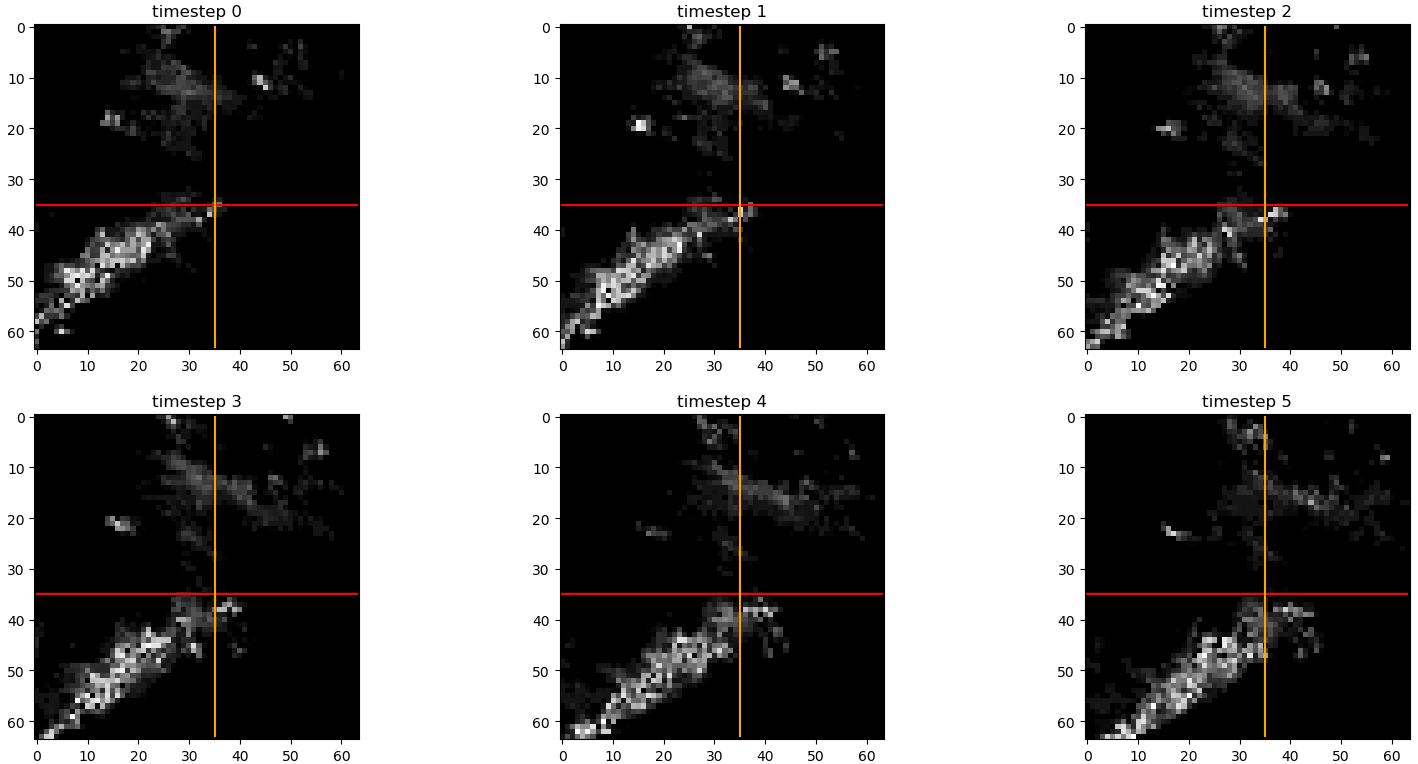
\includegraphics[width=\linewidth]{pics/5Daten_1Label_Radar.png}
	\caption[Beispielhaftes Trainingssample zur vorhersage von 5 Minuten]{Die Grafiken timestep 0 bis timestep 4 sind die 5 eingehenden Daten, die als timestamp 5 bezeichnete Grafik entspricht dem zu lernenden Label. Die Bilder sind jeweils 5 Minuten voneinander entfernte Radarbilder. Die orange und rote Linien dienen nur zur besseren Darstellung der Bewegung.}
	\label{5D1L}
\end{figure}

Die Daten für eine einfache fünfminütliche Vorhersage sind in Abbildung~\ref{5D1L} dargestellt.

Für das Training können allerdings nicht alle Daten verwendet werden. Zum einen, kommt es vor, dass eine Radarstation keine Daten liefert, solche Bilder eignen sich nicht für das Training. Auch kommt es sehr häufig vor, dass kein Regen stattfindet, die Grafik also komplett schwarz und ohne Struktur ist. Auch solche Samples sind nicht zum Training geeignet. Als letzte Einschränkung gilt, dass über alle fünf eingehenden Zeitschritte ein Mindestmaß an Regen zu sehen sein muss um in das Trainingsset aufgenommen zu werden. Für die Label gibt es keine Einschränkung, da sowohl die Fortbewegung von Regen, als auch das verschwinden gelernt werden soll. Jeder Zeitschritt wird maximal einmal in das Trainingsset aufgenommen, was einmal als Label verwendet wurde, wird keinesfalls in einem anderen Sample als als Eingabedatum verwendet. Beim Aufteilen des Sets zwischen Trainings und Validierungsset ist es wichtig, dass nicht zufällige Samples ausgewählt werden, damit garantiert ist, dass keine ähnliche Wetterlage bereits gesehen wurde.
Die so entstandenen Daten werden vor Eingabe in das Netz noch auf Werte zwischen 0 und 1 Normiert. Ab jetzt können die Daten für das Trainieren verwendet werden.


\subsection{Herausforderungen in diesem Kapitel}
Die größte Herausforderung in diesem Kapitel war zweifelsfrei die große Datenmenge, die wir verarbeitet haben. Die Rohdaten der 18 Jahre in 5-Minuten-Auflösung hätte unseren zugewiesenen Speicher gesprengt. Mit Btrfs, das die Dateien on-the-fly komprimiert und de-dupliziert, passten die Daten doch auf unsere Festplatte. Auch mussten wir eventuelle Ausreißer empirisch entfernen, weil das Berechnen des Histogramm über so viele Daten zu aufwendig wäre.

Darüber hinaus lagen die Archive des DWD im Tar-Format vor, das keine Checksumme anbietet und somit erst beim Entpacken bemerkt werden kann, dass beim Download einer Datei ein Fehler auftrat. Bei den großen Tar-Archiven des DWD ist leider mehrmals ein Download-Fehler aufgetreten, der sehr spät auffiel.
